\chapter{基于深度学习的多实例点云配准}
现有的工作主要集中在单对单的物体或场景同级别的点云配准,该方向上的工作已经十分成熟,传统的ICP配准方法\cite{barath2021progressive, li2020evaluation, shi2020improved}和深度学习方法\cite{qin2022geometric,barath2019progressive,barath2021progressive}都能达到很好的效果。但是,目前的工作对于物体对场景中多个物体的不同级别的多个配准表现仍然有待提升。本文主要构建了一种基于对应聚类方法的多实例点云配准模型和一种基于对比学习的多实例点云配准模型,将在本章展开讨论。
\section{问题陈述}

在多实例点云配准问题中,源点云$\mathbf{X}$提供了一个3D模型的实例,目标点云$\mathbf{Y}$包含了这个模型的$K$个实例,其中这些实例是一组点的集合,这些点可能只采样了3D模型的一部分。如果我们将第$k^{th}$个实例写为$\mathbf{Y}_k$,那么目标点云$\mathbf{Y}$可以分解为$
%\begin{equation}
\mathbf{Y} = \mathbf{Y}_0 \cup \mathbf{Y}_1 \cup \ldots \mathbf{Y}_k \ldots \cup \mathbf{Y}_K$。
%\end{equation}
这里我们使用$\mathbf{Y}_0$表示点云中不属于任何实例的部分。
多实例3D配准的目标是找到刚性变换$(\mathbf{R}_k, \mathbf{t}_k)$,将源实例$\mathbf{X}$对准到每个目标实例$\mathbf{Y}_k$。
如果我们设法获得源实例与每个目标实例$\mathbf{X} \leftrightarrow \mathbf{Y}_k$之间的对应关系,那么通过最小化对齐误差之和(\ref{eq:solve_rigid_transform}) \cite{SVD},可以从对应关系集合$\mathbf{X}\leftrightarrow \mathbf{Y}_k$中求解目标点云中第$k^{th}$个实例的位姿$(\mathbf{R}_k, \mathbf{t}_k)$:
\begin{equation}
\underset{\mathbf{R}_k,\mathbf{t}k}{\min}\sum_i{\parallel}\mathbf{y}{ki}-(\mathbf{R}_k\mathbf{x}_i+\mathbf{t}_k)\parallel ^2.
\label{eq:solve_rigid_transform}
\end{equation}
考虑到我们已经获得了源点云和目标点云之间的一组对应关系$\mathcal{C}$。多实例配准任务的关键是将这些对应关系分类为与不同实例相关的独立集合,即:
\begin{equation}
\mathcal{C} = \mathcal{C}_0 \cup \mathcal{C}_1\cdots \cup \mathcal{C}_K.
\end{equation}
这里,$\mathcal{C}_0$用来表示异常值集合。如我们所见,多实例配准不仅需要剔除异常值对应关系,还需要解决来自不同实例的对应关系的歧义。这个任务并不容易,因为所有实例看起来都一样,而且通常存在大量的异常值对应关系。

\section{高效对应聚类的多实例点云配准}

\subsection{结构模型}
我们提出的方法的概述如图\ref{fig:multicluster}所示。我们的方法以点对应关系作为输入。接着通过检查对应关系之间的距离一致性来构建一个不变性一致性矩阵。然后,通过将列或行向量视为这些对应关系的“特征”,将这些对应关系快速聚类成不同的组。通过凝聚聚类方法高效地进行聚类,然后通过交替合并相似的变换和重新分配簇标签进行多次迭代来进一步优化。在对应关系数量较大的情况下,我们可以选择性地应用降采样和上采样过程。详细内容将在接下来的章节中介绍。

\begin{figure*}[ht]
    \centering
    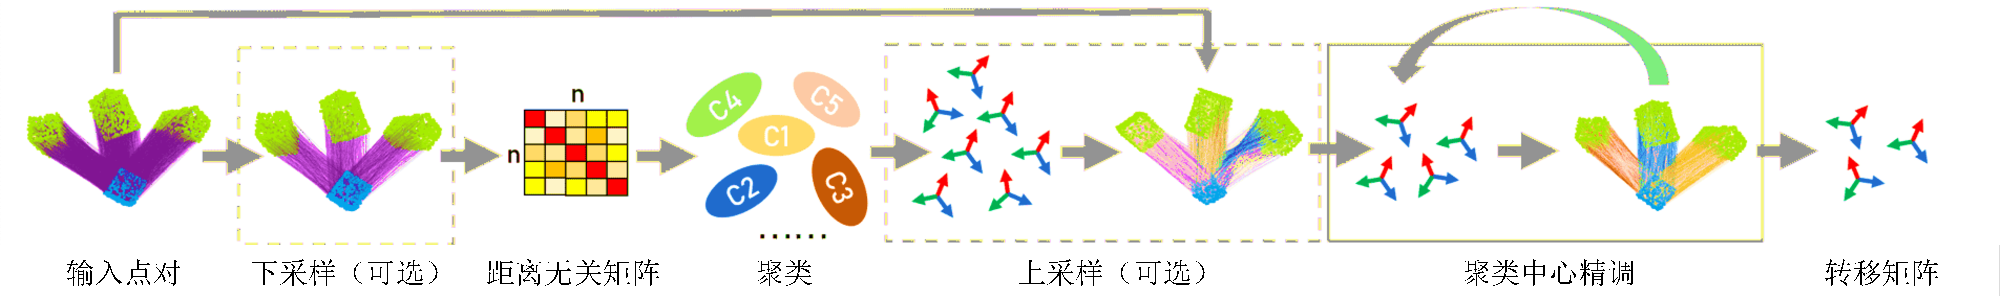
\includegraphics[width=1\textwidth]{images/multi-cluster.pdf} % Reduce the figure size so that it is slightly narrower than the column. Don't use precise values for figure width.This setup will avoid overfull boxes.
    \caption{我们提出的多实例点云配准方法的流程。从输入对应关系构建距离不变性矩阵,用于将对应关系聚类为不同的簇(\textbf{聚类}),并进行优化(\textbf{簇优化})。最后,从每个对应关系簇中估计与每个实例相关的刚体变换(\textbf{变换})。为了处理大量的对应关系,采用两个附加过程(\textbf{下采样}和\textbf{上采样})。}
    \label{fig:multicluster}
    \vspace{-0.6in}
\end{figure*}

\subsection{基于不变型矩阵的聚类}
\label{subsec:Distance-Consistency-Graph}
距离不变性特性在3D配准领域已经被研究多年\cite{yang2020teaser, shi2021robin,leordeanu2005spectral},该特性描述了在刚性变换之后两点之间的距离保持不变。具体来说,如果 $c_i :\mathbf{x}_i \leftrightarrow \mathbf{y}_i$ 和 $c_j : \mathbf{x}_j \leftrightarrow \mathbf{y}_j$ 是两个真实的对应关系,那么它们应该满足
%
\begin{equation}
G_{ij}=|d_{ij} - d'_{ij} | < \delta
\label{eq:abs_diff}
\end{equation}
其中 $d_{ij} = |\mathbf{x}_i-\mathbf{x}_j|, d'{ij}=|\mathbf{y}_i -\mathbf{y}_j|$,$\delta $ 是一个用于考虑噪声的阈值。
因此,$d_{ij}$ 和 $d'_{ij}$ 之间的差异可以用作度量是否存在异常值,或者两个对应关系是否来自不同的刚性变换的指标。我们参考\cite{matrix},使用相对差异作为度量,而不是在(\ref{eq:abs_diff})中定义的绝对差异,
\begin{equation}
G_{ij} = s_{ij}^2, s_{ij} = \min( \frac{d_{ij}}{d'_{ij}}, \frac{d'_{ij}}{d_{ij}}) \in (0, 1).
\end{equation}
通过计算所有对应关系对之间的分数,可以获得一个\emph{距离不变性矩阵} $G$(我们令 $G_{ii} = 1$)。距离不变性矩阵是对称的,其中每一列或行是一个向量,描述了给定对应关系与其他对应关系之间的兼容性\cite{reviewof3dourlierremovingjiaqiYang}。

我们将列向量 $G_i = (G_{i1}, \ldots , G_{ij}, \ldots)^T$ 称为对应关系 $c_i$ 的\emph{兼容性向量}。
我们观察到,如果两个对应关系属于同一个实例,它们的\emph{兼容性向量}具有相似的模式。
考虑两个对应关系 $c_i, c_j \in \mathcal{C}s$。对于任何对应关系 $c_k \in \mathcal{C}s$,由于距离不变性,我们有 $G_{ik} \rightarrow 1, G_{jk} \rightarrow 1$。对于其他对应关系 $c_k \in \mathcal{C}/\mathcal{C}s$,我们可能有 $G_{ik} \rightarrow 0, G_{jk} \rightarrow 0$。换句话说,$G_i,G_j$ 具有相似的 $0-1$ 模式。
相比之下,如果两个对应关系属于不同的实例,它们的兼容性向量则非常不同。

对应关系的兼容性向量可以被视为该对应关系的特征表示或“特征”。属于同一刚性变换的对应关系具有相似的特征。因此,基于这些兼容性向量,我们可以将对应关系聚类为与来自不同实例的内点相关的不同组。

\subsubsection{快速对应关系聚类.}
我们以自底向上的方式聚类对应关系,这比现有方法采用的谱聚类\cite{parra2019practical}\cite{shi2021robin}要快得多。一开始,每个对应关系被视为一个独立的组。然后,我们反复合并距离最小的两个组,直到两个组之间的最小距离大于给定值($min dist thresh$)。定义组之间距离的方式产生了不同风格的算法。我们遵循\cite{Tlinkage}来定义距离。设$\mathbf{p}_i, \mathbf{p}_j$为两个组$i$和$j$的表示向量,组距离定义为
\begin{equation}
d(\mathbf{p}_i, \mathbf{p}_j)= 1-\frac{\langle \mathbf{p}_i,\mathbf{p}_j\rangle}{\parallel \mathbf{p}_i\parallel ^2+\parallel \mathbf{p}_j\parallel ^2-\langle \mathbf{p}_i,\mathbf{p}_j\rangle}.
\end{equation}
如果两个组合并,新组的表示向量更新为
$\mathbf{p}_i \leftarrow \min (\mathbf{p}_i, \mathbf{p}_j),$ 其中 $\min(\cdot)$ 表示取两个向量每个维度的最小值。
在聚类开始时,一个组(只包含一个对应关系)的表示向量设置为该对应关系的兼容性向量。

\subsubsection{递归簇细化.}
\label{sec:cluster_refinement}
在凝聚聚类之后,我们通过重复以下步骤来进一步优化结果,直到没有变化发生。

步骤1. 从对应关系数量大于阈值 $\alpha$ 的簇中估计刚性变换。

步骤2. 合并相似的变换。这一步将在下一节中解释。

步骤3. 为每个对应关系重新分配簇标签。将每个对应关系分配给对齐误差最小的变换。如果在所有变换中最小的对齐误差大于 $inlier_thresh$,则将对应关系标记为异常值。

在迭代过程中,对应关系变得越来越集中,因此我们可以在步骤1中调整 $\alpha$ 以增加异常值拒绝的强度。我们在每次迭代中更新 $\alpha$ 的策略如下:
\begin{equation}
\alpha \leftarrow \min(\alpha _0\times \theta ^{n-1},\left[N/100 \right] ),
\label{eq:alpha}
\end{equation}
其中 $n$ 表示第 $n^{th}$ 次迭代,$N$ 是对应关系的数量,$\left[ \cdot \right]$ 是四舍五入运算。在我们的实验中,我们设置 $\alpha_0 = 3$ 和 $\theta = 3$。细化过程通常在我们的实验中在三次迭代内收敛,因此效率也非常高。

\subsubsection{合并重复变换.}
有时来自不同簇的相似变换会生成,这意味着它们可能属于同一个实例。在这种情况下,我们需要合并它们。
给定两个估计的变换 $(\mathbf{R}1, \mathbf{t}1)$ 和 $(\mathbf{R}2, \mathbf{t}2)$,我们计算每个对应关系的对齐误差,即 $e{ki} = |\mathbf{y}{i}-(\mathbf{R}k \mathbf{x}{i} + \mathbf{t}k)|^2, (k = 1,2)$。接下来,我们设置 $p{ki} = 1$ 如果 $e{ki} < inlier_thresh$,否则 $p{ki}=0$。因此,我们为两个变换获得两个二进制集 $P_1, P_2$。合并两个变换的条件是
\begin{equation}
IOU = |P_1 \cap P_2|/|P_1 \cup P_2| \geq 80%.
\label{eq:iou}
\end{equation}
如果满足这个条件,我们将放弃一个异常值较多的变换($p_{ki} = 0$)。然后我们根据在所有变换中对齐误差最小的一个重新为每个对应关系分配簇标签。

\subsubsection{从簇中提取变换.}
在聚类之后,我们需要从这些对应关系簇中提取刚性变换。由于我们不知道目标点云中真实实例的数量,因此我们需要自动选择那些内点簇。我们首先选择内点簇的元素数量大于阈值(在我们的实验中为 $10$)并从这些簇中估计变换。接下来,我们根据其内点数量按降序对变换进行排序。一个变换拥有的内点越多,它与真实实例相关联的可能性就越高。最后,我们检查内点数量在变换之间的降低比例,以及第一个变换(具有最多内点)之间的比例,通过
\begin{equation}
    \gamma_k = \#I_{k}/\#I_{0},\,\, k = 1,2,\ldots
\end{equation}

其中 $\#I_k$ 表示第 $k^{th}$ 变换的内点数量。如果 $\gamma_k <= \gamma_{thresh}$,我们忽略所有在 $k$ 之后的变换。$\gamma_{thresh}$ 可以更改以在召回和精确度之间进行权衡。

\subsubsection{处理大量对应关系.}
% TODO down_sample and cluster
% 1.unsample
% 为什么要downsample,downsample为什么可行
当输入对应关系的数量很大时,计算距离不变矩阵和聚类对应关系可能会变得昂贵。我们通过添加下采样和上采样过程来解决这个问题。在构建距离不变矩阵之前进行下采样过程,通过随机抽样固定数量的对应关系(在我们的实现中为 $1024$)进行进一步处理。在选定对应关系聚类之后进行上采样过程,将所有对应关系分配给现有簇。分配是通过选择对齐误差最小的变换来完成的,如第 \ref{sec:cluster_refinement} 节中的步骤3所述。

\subsection{训练过程}

\subsection{推理过程}

\section{基于深度学习的多实例点云配准}
\subsection{对比学习}
\subsection{网络结构}
\subsection{损失函数}
\subsection{训练过程}
\subsection{推理过程}

\section{实验结果与分析}
\subsection{数据集与硬件细节}
\subsection{整体配准效果}
\subsection{配准量化结果}
\subsection{配准可视化结果}
\subsection{消融实验}

\section{小结}